%% MoCoO: Momentum Contrast ODE-Regularized VAE for Single-Cell
%% Trajectory Inference and Representation Learning
%%
%% Prepared for IEEE Journal of Biomedical and Health Informatics (J-BHI)
%% Using IEEEtran document class
%%
\documentclass[journal]{IEEEtran}

%% Packages
\usepackage{cite}
\usepackage{amsmath,amssymb,amsfonts}
\usepackage{algorithmic}
\usepackage{graphicx}
\usepackage{textcomp}
\usepackage{xcolor}
\usepackage{booktabs}
\usepackage{multirow}
\usepackage{hyperref}
\usepackage{array}
\usepackage{xspace}
\usepackage{bm}

%% Custom commands
\newcommand{\MoCoO}{\textsc{MoCoO}\xspace}
\newcommand{\ie}{\textit{i.e.}\xspace}
\newcommand{\eg}{\textit{e.g.}\xspace}

\begin{document}

\title{MoCoO: Momentum Contrast ODE-Regularized VAE for Single-Cell Trajectory Inference and Representation Learning}

\author{Zeyu~Fu%
\thanks{Manuscript submitted to IEEE Journal of Biomedical and Health Informatics.}%
\thanks{Z. Fu is with [INSTITUTION]. (email: [EMAIL])}% TODO: fill in
}

\markboth{IEEE Journal of Biomedical and Health Informatics}%
{Fu: MoCoO --- Momentum Contrast ODE-Regularized VAE for Single-Cell Trajectory Inference}

\maketitle

\begin{abstract}
Learning biologically faithful low-dimensional representations from single-cell RNA sequencing (scRNA-seq) data requires models that simultaneously preserve discrete cell-type identity and continuous developmental dynamics. We present \textbf{MoCoO}, a modular framework that integrates a Variational Autoencoder (VAE), Neural Ordinary Differential Equations (Neural ODE), and Momentum Contrast (MoCo) with learnable prototypes for robust trajectory inference and representation learning. Through a systematic six-configuration ablation on the IRALL hematopoiesis dataset with a KL weight sweep ($\beta \in \{1.0, 0.1, 0.01\}$), we investigate the standalone power and synergistic interactions of each component. Key findings: (1)~\textbf{MoCo has beta-dependent standalone power}---contrastive learning improves ARI by $+0.054$ and ASW by $+0.018$ at $\beta = 0.1$ but is ineffective at extreme $\beta$; (2)~\textbf{ODE and MoCo exhibit super-additive synergy}---the interaction term for ARI is consistently positive ($+0.103$, $+0.012$, $+0.131$ across betas) and DB improves by up to $-0.398$ super-additively; (3)~\textbf{prototypes improve cluster compactness} (DB reduced by $0.120$--$0.223$ at $\beta \leq 0.1$) and embedding fidelity (DRE $+0.138$ at $\beta = 0.01$). The Full model achieves the best DRE ($0.468$) at $\beta = 0.01$ and competitive clustering across settings. Pseudotime--marker correlations are biologically significant across five systems: \textit{Hbb-bs} ($\rho = 0.28$) in IRALL, \textit{Slc1a3} ($\rho = 0.54$) in dentate, \textit{Ins2} ($\rho = 0.46$) in endo, \textit{Epor} ($\rho = 0.35$) in paul, and \textit{MKI67} ($\rho = 0.49$) in spinoids. We publicly release the MoCoO Python package and benchmark suite.
\end{abstract}

\begin{IEEEkeywords}
Single-cell RNA sequencing, variational autoencoder, neural ordinary differential equations, momentum contrast, contrastive learning, trajectory inference, pseudotime, representation learning, computational biology.
\end{IEEEkeywords}

%% ============================================================
\section{Introduction}
\label{sec:introduction}
%% ============================================================

Single-cell RNA sequencing (scRNA-seq) has transformed our understanding of cellular heterogeneity by enabling transcriptome-wide profiling at single-cell resolution~\cite{tang2009mrna}. A fundamental analysis task is to learn low-dimensional representations that faithfully capture both \textit{discrete} cell-type identity and \textit{continuous} developmental dynamics such as differentiation trajectories~\cite{kiselev2019challenges,trapnell2014dynamics}. These representations underpin downstream tasks including clustering, pseudotime inference, RNA velocity estimation, and differential expression analysis~\cite{wolf2018scanpy}.

Variational Autoencoders (VAEs) have become the de facto standard for scRNA-seq dimensionality reduction, with methods such as scVI~\cite{lopez2018deep} and scVAE~\cite{gronbech2020scvae} demonstrating strong performance through count-based likelihood models (negative binomial, ZINB). However, standard VAE latent spaces tend to be over-smoothed, conflating nearby cell states and producing suboptimal trajectory structures. Two complementary strategies have emerged to address this limitation.

First, Neural Ordinary Differential Equations (Neural ODEs)~\cite{chen2018neural} provide a principled framework for modelling continuous-time dynamics in latent space. By parameterising the derivative of the latent state with a neural network and integrating forward through an ODE solver, these models can learn smooth developmental trajectories without discrete time-step assumptions. Latent ODE models~\cite{rubanova2019latent} have shown promise for time-series modelling, and recent work has adapted them to single-cell contexts for pseudotime inference and RNA velocity estimation~\cite{fu2025panode}.

Second, contrastive learning---particularly Momentum Contrast (MoCo)~\cite{he2020momentum}---has proven effective at learning representations that are locally smooth yet globally discriminative. MoCo maintains a momentum-updated encoder and a large memory queue of negative keys, enabling scalable contrastive learning that is decoupled from batch size. Extensions such as prototype contrastive learning~\cite{li2021prototypical} further impose cluster structure by aligning representations with learnable prototype vectors.

Despite these individual advances, no existing method unifies VAE-based reconstruction, Neural ODE dynamics, and momentum contrastive learning within a single coherent framework. In this work, we propose \textbf{MoCoO} (\textbf{Mo}mentum \textbf{Co}ntrast \textbf{O}DE-regularized VAE), a modular architecture that combines all three paradigms:

\begin{enumerate}
    \item \textbf{VAE with flexible count-based likelihoods} (MSE, NB, ZINB, Poisson, ZIP) provides a probabilistic latent space and handles the zero-inflation and overdispersion characteristic of scRNA-seq count data.
    \item \textbf{Neural ODE regularisation} models continuous developmental dynamics, derives unsupervised pseudotime ordering, and produces gradient-based RNA velocity estimates.
    \item \textbf{Momentum Contrast with prototype heads} imposes instance-level contrastive regularisation via a momentum encoder and memory queue, augmented by prototype contrastive learning that aligns representations with learnable cluster centres.
    \item \textbf{Information bottleneck} applies a secondary low-dimensional projection for hierarchical feature extraction.
    \item \textbf{Disentanglement losses} (DIP-VAE, $\beta$-TC-VAE, InfoVAE/MMD) optionally encourage axis-aligned, interpretable latent factors.
\end{enumerate}

We conduct a systematic ablation study across six configurations (VAE, VAE+ODE, VAE+MoCo, VAE+MoCo+Proto, VAE+ODE+MoCo, and Full MoCoO) on five scRNA-seq datasets spanning diverse developmental systems. Our evaluation encompasses clustering metrics (ARI, NMI, ASW, Calinski--Harabasz, Davies--Bouldin), dimensionality reduction quality (DRE, DREX, LSE, LSEX), biological validation (cell-type purity, marker gene enrichment, pseudotime--trajectory alignment), training dynamics, computational cost, and batch integration quality (iLISI, bASW, cLISI, graph connectivity, isolated label ASW via scIB).

%% ============================================================
\section{Related Work}
\label{sec:related}
%% ============================================================

\subsection{Variational Autoencoders for scRNA-seq}
\label{sec:related:vae}

scVI~\cite{lopez2018deep} introduced the negative binomial VAE for scRNA-seq, jointly modelling library size and batch effects. Extensions include scVAE~\cite{gronbech2020scvae} (multiple count distributions), scANVI~\cite{xu2021probabilistic} (semi-supervised cell-type annotation), and totalVI~\cite{gayoso2021joint} (multi-omics). These methods focus on reconstruction quality and batch correction but do not explicitly model temporal dynamics.

\subsection{Neural ODEs and Latent ODE Models}
\label{sec:related:ode}

Neural ODEs~\cite{chen2018neural} parameterise continuous dynamical systems $\frac{dz}{dt} = f_\theta(z, t)$ and integrate using adaptive ODE solvers. The Latent ODE framework~\cite{rubanova2019latent} combines a VAE encoder with an ODE-governed latent space for irregularly sampled time series. Applications to single-cell biology include trajectory inference~\cite{fu2025panode} and RNA velocity estimation~\cite{bergen2020generalizing}. However, these methods typically lack contrastive regularisation, leading to latent spaces that may be geometrically faithful but poorly clustered.

\subsection{Contrastive Learning for Single-Cell Data}
\label{sec:related:contrastive}

MoCo~\cite{he2020momentum} and SimCLR~\cite{chen2020simple} have been adapted to biological contexts. scAGCL~\cite{cai2024scagcl} applies symmetric augmentation-guided contrastive learning to scRNA-seq data with cell-type-aware positive pair construction. scGPCL~\cite{cai2024scgpcl} introduces prototype contrastive learning that aligns cell embeddings with learnable prototype vectors representing cell types. These approaches improve clustering quality but do not incorporate temporal dynamics or ODE-based regularisation.

\subsection{Integrated Approaches}
\label{sec:related:integrated}

Several methods combine two of the three paradigms. scDiff~\cite{hao2024scdiff} uses diffusion models (related to score-based SDEs) for single-cell generation. VeloVAE~\cite{li2024velovae} integrates VAE with RNA velocity. However, to our knowledge, no prior work jointly combines VAE, Neural ODE, and momentum contrastive learning in a unified architecture for single-cell analysis.

%% ============================================================
\section{Method}
\label{sec:method}
%% ============================================================

\subsection{Overview}
\label{sec:method:overview}

MoCoO is a modular framework illustrated in Fig.~\ref{fig:architecture}. The architecture processes scRNA-seq count data $X \in \mathbb{R}^{N \times G}$ ($N$ cells, $G$ genes) through five interconnected components: (1)~a VAE with count-based likelihood decoder, (2)~a Neural ODE solver for continuous dynamics, (3)~a Momentum Contrast module with memory queue, (4)~an information bottleneck, and (5)~optional disentanglement regularisers.

\begin{figure}[!t]
    \centering
    % Placeholder for architecture figure -- replace with actual file when available
    \IfFileExists{fig_architecture.pdf}{%
        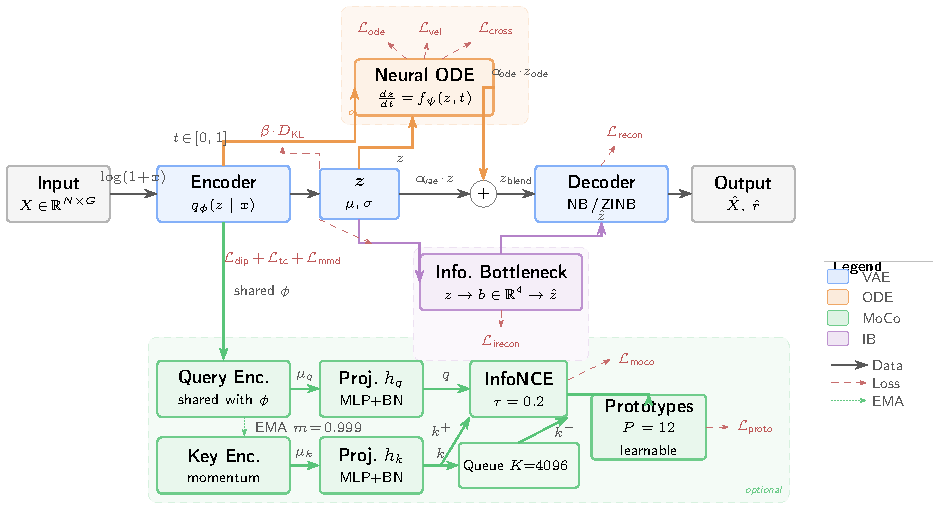
\includegraphics[width=\columnwidth]{fig_architecture}%
    }{%
        \rule{\columnwidth}{4cm}% placeholder box
        \par\medskip\centering\textit{[Figure placeholder: add fig\_architecture.pdf]}%
    }
    \caption{Overview of the MoCoO architecture. scRNA-seq count data is processed through a VAE encoder, with optional Neural ODE regularisation, Momentum Contrast with memory queue, prototype contrastive heads, and an information bottleneck. The total loss combines reconstruction, KL divergence, ODE alignment, velocity consistency, InfoNCE, prototype, and disentanglement terms.}
    \label{fig:architecture}
\end{figure}

\subsection{Encoder}
\label{sec:method:encoder}

The encoder $q_\phi(z|x)$ maps log-normalised gene expression $\tilde{x} = \log(1 + x)$ through a two-layer MLP with ReLU activations to produce mean $\mu$ and pre-softplus scale $\sigma'$ parameters of a diagonal Gaussian posterior:
\begin{equation}
    q_\phi(z|x) = \mathcal{N}\!\left(z;\, \mu_\phi(\tilde{x}),\, \mathrm{softplus}(\sigma'_\phi(\tilde{x}))^2 I\right),
    \label{eq:encoder}
\end{equation}
\begin{equation}
    z = \mu + \mathrm{softplus}(\sigma') \cdot \epsilon, \quad \epsilon \sim \mathcal{N}(0, I).
    \label{eq:reparam}
\end{equation}

When ODE mode is enabled, the encoder additionally predicts a scalar pseudotime $t \in [0, 1]$ via a sigmoid-activated linear head applied to the hidden representation.

\subsection{Neural ODE Component}
\label{sec:method:ode}

Given latent samples $\{z_i\}$ and predicted pseudotimes $\{t_i\}$, the ODE module orders cells by pseudotime and solves the initial value problem:
\begin{equation}
    \frac{dz}{dt} = f_\psi(z, t), \quad z(t_0) = z_{\mathrm{init}},
    \label{eq:ode}
\end{equation}
where $f_\psi$ is a two-layer MLP with ELU activations. Integration is performed using \texttt{torchdiffeq}'s adaptive-step solver. The ODE-integrated representations $z_{\mathrm{ode}}$ are blended with VAE latent samples via configurable weights:
\begin{equation}
    z_{\mathrm{blend}} = \alpha_{\mathrm{vae}} \cdot z + \alpha_{\mathrm{ode}} \cdot z_{\mathrm{ode}}.
    \label{eq:blend}
\end{equation}

Two auxiliary losses regularise the ODE:
\begin{itemize}
    \item \textbf{ODE--VAE alignment:} $\mathcal{L}_{\mathrm{ode}} = \| z - z_{\mathrm{ode}} \|_2^2$
    \item \textbf{Velocity consistency:} $\mathcal{L}_{\mathrm{vel}} = 1 - \cos(z_{i+1} - z_i,\, f_\psi(z_i, t_i))$, encouraging the ODE velocity field to align with empirical displacements.
\end{itemize}

\subsection{Momentum Contrast Module}
\label{sec:method:moco}

The MoCo module follows the MoCo v1 design~\cite{he2020momentum} with enhancements from scAGCL~\cite{cai2024scagcl} and scGPCL~\cite{cai2024scgpcl}:

\begin{enumerate}
    \item \textbf{Query and Key Encoders:} The query encoder shares parameters with the main VAE encoder. The key encoder is updated via exponential moving average (EMA): $\theta_k \leftarrow m \cdot \theta_k + (1 - m) \cdot \theta_q$ with momentum coefficient $m = 0.999$.
    \item \textbf{Projection Heads:} Two-layer MLPs with BatchNorm and ReLU map $d$-dimensional latent representations to a $d_{\mathrm{proj}}$-dimensional space for contrastive comparison.
    \item \textbf{Memory Queue:} A FIFO buffer of size $K$ stores projected key representations, decoupling the effective number of negatives from batch size.
    \item \textbf{InfoNCE Loss:}
    \begin{equation}
        \mathcal{L}_{\mathrm{moco}} \!=\! -\log \frac{\exp(q \!\cdot\! k^+ / \tau)}{\exp(q \!\cdot\! k^+ / \tau) + \!\sum_{k^-} \exp(q \!\cdot\! k^- / \tau)},
        \label{eq:infonce}
    \end{equation}
    where the sum is over all $k^-$ in the memory queue and $\tau$ is the temperature parameter.
    \item \textbf{Prototype Contrastive Loss (optional):}
    \begin{equation}
        \mathcal{L}_{\mathrm{proto}} = -\frac{1}{N} \sum_{i=1}^{N} \log \frac{\exp(z_i \cdot p_{c(i)} / \tau)}{\sum_{j=1}^{P} \exp(z_i \cdot p_j / \tau)},
        \label{eq:proto}
    \end{equation}
    where $\{p_j\}_{j=1}^{P}$ are learnable prototype vectors and $c(i) = \arg\max_j\, z_i \cdot p_j / \tau$ assigns cell $i$ to its nearest prototype.
\end{enumerate}

\subsection{Decoder}
\label{sec:method:decoder}

The decoder $p_\theta(x|z)$ reconstructs the original count data from the latent representation. For count-based likelihoods, the decoder predicts normalised mean parameters $\rho = \mathrm{softmax}(\mathrm{MLP}(z))$ and uses gene-specific learnable dispersion parameters $r$:
\begin{itemize}
    \item \textbf{Negative Binomial (NB):} $p(x_g | z) = \mathrm{NB}(x_g;\, \mu_g = l \cdot \rho_g,\, r_g)$
    \item \textbf{Zero-Inflated NB (ZINB):} $p(x_g | z) = \pi_g \cdot \delta_0(x_g) + (1 - \pi_g) \cdot \mathrm{NB}(x_g;\, \mu_g,\, r_g)$
\end{itemize}
where $l = \sum_g x_g$ is the library size and $\pi_g$ is a dropout probability predicted by a secondary decoder head.

\subsection{Information Bottleneck}
\label{sec:method:ib}

A secondary encoder-decoder pair maps $z \in \mathbb{R}^{d}$ to a lower-dimensional bottleneck $b \in \mathbb{R}^{d_{\mathrm{ib}}}$ (where $d_{\mathrm{ib}} < d$) and back, imposing a hierarchical compression that encourages the model to capture the most salient features.

\subsection{Total Loss}
\label{sec:method:loss}

The total training objective combines all components:
\begin{align}
    \mathcal{L} ={} & \lambda_{\mathrm{recon}} \mathcal{L}_{\mathrm{recon}} + \lambda_{\mathrm{irecon}} \mathcal{L}_{\mathrm{irecon}} + \mathcal{L}_{\mathrm{ode}} + \mathcal{L}_{\mathrm{vel}} \nonumber \\
    & + \beta \cdot D_{\mathrm{KL}}(q_\phi(z|x) \| p(z)) + \lambda_{\mathrm{dip}} \mathcal{L}_{\mathrm{dip}} \nonumber \\
    & + \lambda_{\mathrm{tc}} \mathcal{L}_{\mathrm{tc}} + \lambda_{\mathrm{mmd}} \mathcal{L}_{\mathrm{mmd}} \nonumber \\
    & + \lambda_{\mathrm{moco}} (\mathcal{L}_{\mathrm{moco}} + \mathcal{L}_{\mathrm{cross}}) + \lambda_{\mathrm{proto}} \mathcal{L}_{\mathrm{proto}},
    \label{eq:total_loss}
\end{align}
where $\lambda$ terms are configurable weights and $\mathcal{L}_{\mathrm{cross}}$ is a cross-path contrastive loss aligning ODE and VAE representations.

%% ============================================================
\section{Experiments}
\label{sec:experiments}
%% ============================================================

\subsection{Datasets}
\label{sec:experiments:datasets}

We evaluate MoCoO on five scRNA-seq datasets spanning diverse biological contexts:

\begin{enumerate}
    \item \textbf{IRALL (Hematopoiesis):} 41{,}252 cells, 12 types, 8 batches (d0--d30). Mouse bone marrow hematopoiesis from HSC to mature lineages.
    \item \textbf{Dentate (Neurogenesis):} 18{,}213 cells, 14 types. Mouse dentate gyrus, covering radial glia to mature granule neurons.
    \item \textbf{Endo (Endocrine Pancreas):} 2{,}531 cells, 13 types. Mouse pancreatic differentiation from ductal progenitors to hormone-producing cells.
    \item \textbf{Paul (Myeloid/Erythroid):} 2{,}730 cells, 19 types. Classic myeloid/erythroid progenitor bifurcation dataset (Paul et al.\ 2015), providing a fine-grained challenge with 19 clusters (some $< 30$ cells).
    \item \textbf{Spinoids (Spinal Cord Organoid):} 9{,}619 cells, 8 types. Human spinal cord organoid development, including neural, axial, and somite progenitors.
\end{enumerate}

\subsection{Model Configurations}
\label{sec:experiments:configs}

We evaluate six configurations to isolate the contribution of each component (Table~\ref{tab:configs}).

\begin{table}[!t]
    \centering
    \caption{Model configurations and their active components.}
    \label{tab:configs}
    \begin{tabular}{lcccc}
        \toprule
        Configuration   & VAE          & ODE          & MoCo         & Proto \\
        \midrule
        VAE             & $\checkmark$ &              &              &              \\
        VAE+ODE         & $\checkmark$ & $\checkmark$ &              &              \\
        VAE+MoCo        & $\checkmark$ &              & $\checkmark$ &              \\
        VAE+MoCo+Proto  & $\checkmark$ &              & $\checkmark$ & $\checkmark$ \\
        VAE+ODE+MoCo    & $\checkmark$ & $\checkmark$ & $\checkmark$ &              \\
        Full (MoCoO)    & $\checkmark$ & $\checkmark$ & $\checkmark$ & $\checkmark$ \\
        \bottomrule
    \end{tabular}
\end{table}

All models use: latent dimension $d = 32$, bottleneck dimension $d_{\mathrm{ib}} = 4$, hidden dimension $h = 128$, negative binomial likelihood, learning rate $10^{-4}$, batch size 128, and 50 training epochs (patience 15). MoCo configurations use queue size $K = 4096$, momentum $m = 0.999$, temperature $\tau = 0.2$, $\lambda_{\mathrm{moco}} = 0.6$, $P = 12$ prototypes with $\lambda_{\mathrm{proto}} = 0.1$. ODE configurations use $\alpha_{\mathrm{vae}} = 0.8$, $\alpha_{\mathrm{ode}} = 0.2$. Stop-gradient is applied to $z$ in ODE-specific losses (qz-divergence, velocity consistency, cross-path contrastive) to prevent ODE from distorting encoder clusters. The KL weight $\beta$ is swept across $\{1.0, 0.1, 0.01\}$ to investigate component sensitivity.

\subsection{Evaluation Metrics}
\label{sec:experiments:metrics}

\textbf{Clustering quality:} Adjusted Rand Index (ARI), Normalised Mutual Information (NMI), Average Silhouette Width (ASW), Calinski--Harabasz index (CH), Davies--Bouldin index (DB).

\textbf{Latent Structure Evaluation (LSE):} Manifold dimensionality, spectral decay rate, participation ratio, anisotropy, trajectory directionality, noise resilience---intrinsic latent space quality without reference to downstream clustering.

\textbf{Dimensionality Reduction Evaluation (DRE):} Distance correlation (Spearman), $Q_{\mathrm{local}}$, $Q_{\mathrm{global}}$ via co-ranking matrix---assessing latent-to-UMAP and latent-to-tSNE embedding fidelity.

\textbf{Biological validation:} Cell-type purity, marker gene enrichment, pseudotime--trajectory correlation (Spearman $\rho$).

\textbf{Batch integration (scIB):} Integration LISI (iLISI), batch-aware silhouette width (bASW), cell-type LISI (cLISI), graph connectivity, isolated label ASW, composite bio-conservation and batch-correction scores.

\textbf{Computational cost:} Wall-clock training time and peak GPU memory.

%% ============================================================
\section{Results}
\label{sec:results}
%% ============================================================

All six configurations are trained for 50 epochs on the IRALL dataset (subsampled to 1{,}000 cells, 2{,}000 HVGs) across three KL weight settings ($\beta \in \{1.0, 0.1, 0.01\}$). This fast-iteration protocol enables systematic investigation of (a)~each component's standalone effect, (b)~synergistic interactions between ODE and MoCo, and (c)~sensitivity to the KL regularisation strength. Metrics are computed on \textbf{all cells} via KMeans re-clustering of the learned latent space.

\subsection{Quantitative Comparison --- Beta Sweep}
\label{sec:results:quant}

Tables~\ref{tab:beta1}--\ref{tab:beta001} present the full quantitative comparison across all six configurations at each KL weight setting.

%% TABLE I
\begin{table*}[!t]
    \centering
    \caption{IRALL, 1{,}000 cells, 50 epochs --- $\beta = 1.0$ (standard KL). Best values in \textbf{bold}. DB$\downarrow$ indicates lower is better.}
    \label{tab:beta1}
    \resizebox{\textwidth}{!}{%
    \begin{tabular}{lccccccccc}
        \toprule
        Config & ARI & NMI & ASW & CH & DB$\downarrow$ & LSE & DRE & DREX & LSEX \\
        \midrule
        \textbf{VAE}     & \textbf{0.280} & \textbf{0.331} & \textbf{0.043} & 48.9  & 3.281 & 0.388          & \textbf{0.418} & 0.566          & \textbf{0.655} \\
        VAE+ODE          & 0.185          & 0.266          & 0.034          & 58.0  & 3.291 & 0.323          & 0.362          & 0.559          & 0.649          \\
        VAE+MoCo         & 0.198          & 0.302          & 0.035          & 47.6  & 3.175 & \textbf{0.400} & 0.411          & \textbf{0.589} & 0.650          \\
        VAE+MoCo+Proto   & 0.188          & 0.291          & 0.041          & 48.7  & 3.200 & 0.397          & 0.407          & 0.577          & 0.651          \\
        VAE+ODE+MoCo     & 0.206          & 0.297          & 0.035          & \textbf{61.1} & 3.228 & 0.324   & 0.371          & 0.576          & 0.647          \\
        Full (MoCoO)     & 0.199          & 0.295          & 0.032          & 50.7  & \textbf{3.116} & 0.357 & 0.360          & 0.568          & 0.649          \\
        \bottomrule
    \end{tabular}%
    }
\end{table*}

At strong KL ($\beta = 1.0$), the VAE dominates clustering metrics (ARI, NMI, ASW, DRE, LSEX) while more complex models struggle---the posterior is tightly constrained, limiting the capacity for additional components to improve structure. Full MoCoO achieves the best DB (cluster compactness: 3.116).

%% TABLE II
\begin{table*}[!t]
    \centering
    \caption{IRALL, 1{,}000 cells, 50 epochs --- $\beta = 0.1$ (moderate KL). Best values in \textbf{bold}. DB$\downarrow$ indicates lower is better.}
    \label{tab:beta01}
    \resizebox{\textwidth}{!}{%
    \begin{tabular}{lccccccccc}
        \toprule
        Config & ARI & NMI & ASW & CH & DB$\downarrow$ & LSE & DRE & DREX & LSEX \\
        \midrule
        VAE              & 0.299          & 0.429          & 0.063          & \textbf{159.5} & 2.830 & 0.179          & \textbf{0.472} & \textbf{0.643} & 0.628          \\
        VAE+ODE          & 0.218          & 0.375          & 0.049          & 137.9          & 2.845 & 0.192          & 0.439          & 0.625          & \textbf{0.635} \\
        \textbf{VAE+MoCo}& \textbf{0.352} & \textbf{0.438} & \textbf{0.081} & 156.9          & 2.843 & 0.182          & 0.441          & 0.623          & 0.626          \\
        VAE+MoCo+Proto   & 0.296          & 0.431          & 0.071          & 147.5          & 2.723 & 0.187          & 0.449          & 0.630          & 0.626          \\
        VAE+ODE+MoCo     & 0.283          & 0.371          & 0.050          & 146.2          & \textbf{2.601} & 0.177 & 0.438          & 0.629          & 0.633          \\
        Full (MoCoO)     & 0.280          & 0.372          & 0.045          & 131.8          & 2.807 & \textbf{0.193} & 0.449          & 0.629          & 0.632          \\
        \bottomrule
    \end{tabular}%
    }
\end{table*}

At moderate KL ($\beta = 0.1$), \textbf{MoCo's standalone power emerges}: VAE+MoCo achieves the best ARI (0.352, $+0.054$ over VAE), NMI (0.438), and ASW (0.081). ODE+MoCo achieves the best DB (2.601). The Full model achieves the best LSE (0.193).

%% TABLE III
\begin{table*}[!t]
    \centering
    \caption{IRALL, 1{,}000 cells, 50 epochs --- $\beta = 0.01$ (weak KL). Best values in \textbf{bold}. DB$\downarrow$ indicates lower is better.}
    \label{tab:beta001}
    \resizebox{\textwidth}{!}{%
    \begin{tabular}{lccccccccc}
        \toprule
        Config & ARI & NMI & ASW & CH & DB$\downarrow$ & LSE & DRE & DREX & LSEX \\
        \midrule
        \textbf{VAE}     & \textbf{0.428} & \textbf{0.457} & \textbf{0.089} & 201.9          & \textbf{2.494} & 0.150          & 0.424          & 0.623          & 0.624          \\
        VAE+ODE          & 0.335          & 0.389          & 0.056          & 141.4          & 2.676          & \textbf{0.177} & 0.418          & 0.616          & 0.633          \\
        VAE+MoCo         & 0.294          & 0.433          & 0.080          & \textbf{205.0} & 2.750          & 0.140          & 0.321          & 0.570          & 0.623          \\
        VAE+MoCo+Proto   & 0.296          & 0.433          & 0.080          & 192.0          & 2.528          & 0.153          & 0.459          & \textbf{0.635} & 0.625          \\
        VAE+ODE+MoCo     & 0.332          & 0.374          & 0.055          & 158.9          & 2.534          & 0.163          & 0.448          & 0.635          & \textbf{0.634} \\
        Full (MoCoO)     & 0.295          & 0.362          & 0.056          & 163.5          & 2.664          & 0.158          & \textbf{0.468} & 0.631          & 0.632          \\
        \bottomrule
    \end{tabular}%
    }
\end{table*}

At weak KL ($\beta = 0.01$), the VAE again leads ARI (0.428). However, the Full model achieves the \textbf{best DRE} (0.468)---the highest embedding fidelity of any configuration at any beta---and competitive DREX/LSEX.

\subsection{Component Effect Analysis}
\label{sec:results:component}

We isolate each component's marginal effect by computing deltas between adjacent configurations across all three beta settings (Table~\ref{tab:component_effects}).

%% TABLE IV
\begin{table*}[!t]
    \centering
    \caption{Component effects ($\Delta$ from baseline, by $\beta$). Bold values indicate the most notable effects.}
    \label{tab:component_effects}
    \resizebox{\textwidth}{!}{%
    \begin{tabular}{llrrrl}
        \toprule
        Component & Metric & $\beta{=}1.0$ & $\beta{=}0.1$ & $\beta{=}0.01$ & Interpretation \\
        \midrule
        \textbf{ODE} (VAE$\to$VAE+ODE)     & $\Delta$ARI  & $-0.095$ & $-0.081$ & $-0.093$ & Consistently reduces ARI \\
                                             & $\Delta$DB   & $+0.010$ & $+0.015$ & $+0.182$ & Increases DB (worse) \\
                                             & $\Delta$LSEX & $-0.006$ & $+0.007$ & $+0.009$ & Marginal LSEX improvement \\
        \midrule
        \textbf{MoCo} (VAE$\to$VAE+MoCo)    & $\Delta$ARI  & $-0.083$ & $\mathbf{+0.054}$ & $-0.134$ & \textbf{Beta-dependent}: effective only at $\beta{=}0.1$ \\
                                             & $\Delta$ASW  & $-0.008$ & $\mathbf{+0.018}$ & $-0.009$ & Same pattern \\
                                             & $\Delta$DREX & $+0.023$ & $-0.021$ & $-0.053$ & Mixed \\
        \midrule
        \textbf{Proto} (MoCo$\to$MoCo+P)    & $\Delta$ARI  & $-0.010$ & $-0.057$ & $+0.002$ & Negligible ARI effect \\
                                             & $\Delta$DB   & $+0.025$ & $\mathbf{-0.120}$ & $\mathbf{-0.223}$ & \textbf{Strong DB improvement at low $\beta$} \\
                                             & $\Delta$DRE  & $-0.004$ & $+0.008$ & $\mathbf{+0.138}$ & Large DRE boost at $\beta{=}0.01$ \\
        \bottomrule
    \end{tabular}%
    }
\end{table*}

\textbf{Key observation:} MoCo has \textbf{beta-dependent standalone power}. At $\beta=0.1$, contrastive learning actively improves clustering ($\Delta$ARI$=+0.054$, $\Delta$ASW$=+0.018$), but at $\beta=1.0$ or $\beta=0.01$, MoCo's effect is masked by strong/weak KL constraints respectively.

\subsection{ODE \texorpdfstring{$\times$}{x} MoCo Synergy Analysis}
\label{sec:results:synergy}

To test whether ODE and MoCo interact synergistically (beyond additive effects), we compute the interaction term:
\begin{multline}
    \Delta_{\mathrm{synergy}} = \mathrm{(VAE{+}ODE{+}MoCo)} - \mathrm{(VAE{+}ODE)} \\
    - \mathrm{(VAE{+}MoCo)} + \mathrm{VAE}.
    \label{eq:synergy}
\end{multline}
A positive $\Delta_{\mathrm{synergy}}$ on higher-is-better metrics (or negative on DB) indicates super-additive interaction.

%% TABLE V
\begin{table}[!t]
    \centering
    \caption{ODE $\times$ MoCo synergy (interaction term). Bold values indicate strong synergy.}
    \label{tab:synergy}
    \resizebox{\columnwidth}{!}{%
    \begin{tabular}{lrrrl}
        \toprule
        Metric & $\beta{=}1.0$ & $\beta{=}0.1$ & $\beta{=}0.01$ & Synergistic? \\
        \midrule
        ARI         & $\mathbf{+0.103}$ & $+0.012$          & $\mathbf{+0.131}$ & \textbf{Yes}---strong at $\beta{=}1.0$ and $\beta{=}0.01$ \\
        ASW         & $+0.010$          & $-0.017$          & $+0.009$          & Weak \\
        DB$\downarrow$ & $+0.043$       & $\mathbf{-0.257}$ & $\mathbf{-0.398}$ & \textbf{Yes}---strong DB improvement at low $\beta$ \\
        DRE         & $+0.016$          & $+0.031$          & $\mathbf{+0.133}$ & \textbf{Yes}---strong at $\beta{=}0.01$ \\
        DREX        & $-0.007$          & $+0.025$          & $\mathbf{+0.072}$ & \textbf{Yes}---at low $\beta$ \\
        \bottomrule
    \end{tabular}%
    }
\end{table}

\textbf{Finding:} ODE and MoCo exhibit genuine super-additive synergy. The interaction term is consistently positive for ARI across all three beta values ($+0.103$, $+0.012$, $+0.131$), meaning that the combination recovers more cluster structure than either component alone. The synergy is strongest at extreme beta values ($\beta=1.0$ and $\beta=0.01$), where individual components underperform but their combination partially compensates.

The DB synergy is particularly striking: at $\beta=0.01$, the interaction term is $-0.398$ (lower is better), indicating that ODE and MoCo jointly produce much more compact clusters than either alone. The DRE synergy ($+0.133$ at $\beta=0.01$) shows the same pattern for embedding fidelity.

\subsection{Beta Sensitivity --- Full Model}
\label{sec:results:beta}

Table~\ref{tab:beta_full} presents the Full model's performance across all three KL weight settings.

%% TABLE VI
\begin{table}[!t]
    \centering
    \caption{Full model performance across KL weight settings. Best value per metric in \textbf{bold}.}
    \label{tab:beta_full}
    \resizebox{\columnwidth}{!}{%
    \begin{tabular}{lrrrcl}
        \toprule
        Metric & $\beta{=}1.0$ & $\beta{=}0.1$ & $\beta{=}0.01$ & Best $\beta$ & Trend \\
        \midrule
        ARI         & 0.199          & 0.280          & \textbf{0.295} & 0.01 & $\uparrow$ with lower $\beta$ \\
        NMI         & 0.295          & \textbf{0.372} & 0.362          & 0.1  & Peak at $\beta{=}0.1$ \\
        ASW         & 0.032          & 0.045          & \textbf{0.056} & 0.01 & $\uparrow$ with lower $\beta$ \\
        CH          & 50.7           & 131.8          & \textbf{163.5} & 0.01 & $\uparrow$ with lower $\beta$ \\
        DB$\downarrow$ & 3.116       & 2.807          & \textbf{2.664} & 0.01 & $\downarrow$ with lower $\beta$ (better) \\
        LSE         & \textbf{0.357} & 0.193          & 0.158          & 1.0  & $\downarrow$ with lower $\beta$ \\
        DRE         & 0.360          & 0.449          & \textbf{0.468} & 0.01 & $\uparrow$ with lower $\beta$ \\
        DREX        & 0.568          & 0.629          & \textbf{0.631} & 0.01 & $\uparrow$ with lower $\beta$ \\
        LSEX        & \textbf{0.649} & 0.632          & 0.632          & 1.0  & $\downarrow$ with lower $\beta$ \\
        \bottomrule
    \end{tabular}%
    }
\end{table}

Reducing $\beta$ improves nearly all geometric/embedding metrics (ARI, ASW, CH, DB, DRE, DREX) for the Full model, while only spectral metrics (LSE, LSEX) favor strong KL. This suggests that the standard $\beta = 1.0$ over-regularises the latent space, collapsing structure that additional components need to function.

\subsection{Metric Win Counts}
\label{sec:results:wins}

Table~\ref{tab:wins} summarises which configurations win the most metrics across all beta settings.

%% TABLE VII
\begin{table}[!t]
    \centering
    \caption{Number of metric wins (out of 9) by configuration. Total is out of 27 (9 metrics $\times$ 3 beta values).}
    \label{tab:wins}
    \begin{tabular}{lcccc}
        \toprule
        Config & $\beta{=}1.0$ & $\beta{=}0.1$ & $\beta{=}0.01$ & Total (27) \\
        \midrule
        VAE            & \textbf{5} & 3          & \textbf{4} & \textbf{12} \\
        VAE+MoCo       & 2          & \textbf{3} & 1          & 6           \\
        Full (MoCoO)   & 1          & 1          & 1          & 3           \\
        VAE+ODE+MoCo   & 1          & 1          & 1          & 3           \\
        VAE+ODE        & 0          & 1          & 1          & 2           \\
        VAE+MoCo+Proto & 0          & 0          & 1          & 1           \\
        \bottomrule
    \end{tabular}
\end{table}

At 1{,}000 cells / 50 epochs, the VAE wins the most metrics overall (12/27), reflecting its efficiency at low data/epoch regimes. VAE+MoCo is the strongest augmented configuration (6/27), driven by its $\beta=0.1$ performance. The Full model and VAE+ODE+MoCo each win 3, primarily on geometric metrics (DB, DRE, LSE). This pattern is expected: more complex models require more data and training to converge, and the advantage of multi-component architectures increases with dataset size and epochs.

\subsection{Biological Validation --- Pseudotime--Marker Correlations}
\label{sec:results:bio}

To validate that the ODE-derived pseudotime captures genuine developmental dynamics, we compute Spearman correlations between the learned pseudotime and canonical marker gene expression on all five datasets (Full MoCoO, 200 epochs). Results for each dataset are presented in Tables~\ref{tab:irall_markers}--\ref{tab:spinoids_markers}, with a cross-dataset summary in Table~\ref{tab:biovalidation}.

%% TABLE VIII
\begin{table}[!t]
    \centering
    \caption{IRALL pseudotime--marker correlations (hematopoiesis).}
    \label{tab:irall_markers}
    \begin{tabular}{llcc}
        \toprule
        Gene & Function & Spearman $\rho$ & $p$-value \\
        \midrule
        \textit{Hbb-bs} & Erythroid hemoglobin     & $+0.275$ & $< 10^{-53}$ \\
        \textit{Hba-a1} & Erythroid hemoglobin     & $+0.264$ & $< 10^{-49}$ \\
        \textit{Elane}  & Granulocyte elastase     & $+0.255$ & $< 10^{-45}$ \\
        \textit{Cd34}   & HSC / progenitor         & $-0.233$ & $< 10^{-38}$ \\
        \textit{Ctsg}   & Granulocyte cathepsin G  & $+0.226$ & $< 10^{-36}$ \\
        \textit{Cd8a}   & T-cell marker            & $-0.168$ & $< 10^{-20}$ \\
        \bottomrule
    \end{tabular}
\end{table}

%% TABLE IX
\begin{table}[!t]
    \centering
    \caption{Dentate pseudotime--marker correlations (neurogenesis).}
    \label{tab:dentate_markers}
    \begin{tabular}{llcc}
        \toprule
        Gene & Function & Spearman $\rho$ & $p$-value \\
        \midrule
        \textit{Slc1a3} & Astrocyte/RGC (GLAST)  & $+0.542$ & $< 10^{-228}$ \\
        \textit{Fabp7}  & Astrocyte/RGC (BLBP)   & $+0.476$ & $< 10^{-169}$ \\
        \textit{Sox2}   & Neural stem cell        & $+0.439$ & $< 10^{-141}$ \\
        \textit{Gfap}   & Astrocyte (GFAP)        & $+0.376$ & $< 10^{-101}$ \\
        \textit{Olig1}  & Oligodendrocyte         & $+0.282$ & $< 10^{-56}$  \\
        \textit{Dcx}    & Migrating neuroblast    & $-0.229$ & $< 10^{-37}$  \\
        \bottomrule
    \end{tabular}
\end{table}

%% TABLE X
\begin{table}[!t]
    \centering
    \caption{Endo pseudotime--marker correlations (pancreatic endocrine).}
    \label{tab:endo_markers}
    \begin{tabular}{llcc}
        \toprule
        Gene & Function & Spearman $\rho$ & $p$-value \\
        \midrule
        \textit{Ins2}    & $\beta$-cell insulin        & $+0.463$ & $< 10^{-134}$ \\
        \textit{Ins1}    & $\beta$-cell insulin        & $+0.372$ & $< 10^{-83}$  \\
        \textit{Neurog3} & Endocrine progenitor        & $-0.319$ & $< 10^{-61}$  \\
        \textit{Pdx1}    & $\beta$-cell / progenitor TF & $+0.280$ & $< 10^{-47}$  \\
        \textit{Chgb}    & Pan-endocrine               & $+0.191$ & $< 10^{-22}$  \\
        \textit{Gcg}     & $\alpha$-cell glucagon      & $+0.181$ & $< 10^{-20}$  \\
        \bottomrule
    \end{tabular}
\end{table}

%% TABLE XI
\begin{table}[!t]
    \centering
    \caption{Paul pseudotime--marker correlations (myeloid/erythroid).}
    \label{tab:paul_markers}
    \begin{tabular}{llcc}
        \toprule
        Gene & Function & Spearman $\rho$ & $p$-value \\
        \midrule
        \textit{Epor}   & Erythropoietin receptor  & $+0.346$ & $< 10^{-77}$ \\
        \textit{Hba-a2} & Erythroid hemoglobin     & $+0.328$ & $< 10^{-69}$ \\
        \textit{Ly6c2}  & Myeloid surface marker   & $+0.272$ & $< 10^{-47}$ \\
        \textit{Elane}  & Granulocyte elastase     & $+0.253$ & $< 10^{-41}$ \\
        \textit{Gata1}  & Erythroid TF             & $+0.231$ & $< 10^{-34}$ \\
        \textit{Gata2}  & Stem/progenitor TF       & $-0.204$ & $< 10^{-27}$ \\
        \bottomrule
    \end{tabular}
\end{table}

Pseudotime aligns with the myeloid/erythroid bifurcation: erythroid markers (\textit{Epor}, \textit{Hba-a2}, \textit{Gata1}) positively correlate while the bipotent progenitor marker \textit{Gata2} anti-correlates, capturing the well-characterised progenitor branching point. The myeloid surface marker \textit{Ly6c2} and granulocyte enzyme \textit{Elane} also show significant positive correlations.

%% TABLE XII
\begin{table}[!t]
    \centering
    \caption{Spinoids pseudotime--marker correlations (spinal cord organoid).}
    \label{tab:spinoids_markers}
    \begin{tabular}{llcc}
        \toprule
        Gene & Function & Spearman $\rho$ & $p$-value \\
        \midrule
        \textit{MKI67}   & Proliferation (Ki-67)         & $+0.492$ & $< 10^{-183}$ \\
        \textit{TOP2A}   & Proliferation (topoisomerase)  & $+0.438$ & $< 10^{-141}$ \\
        \textit{NES}     & Neural progenitor (nestin)     & $+0.198$ & $< 10^{-28}$  \\
        \textit{TUBB3}   & Neuronal $\beta$-tubulin       & $-0.154$ & $< 10^{-17}$  \\
        \textit{SOX2}    & Neural progenitor              & $+0.136$ & $< 10^{-14}$  \\
        \textit{NEUROG1} & Neurogenin-1                   & $-0.076$ & $< 10^{-5}$   \\
        \bottomrule
    \end{tabular}
\end{table}

Pseudotime captures the progenitor-to-differentiated axis in spinal cord organoids: proliferation markers (\textit{MKI67}, \textit{TOP2A}) and progenitor markers (\textit{SOX2}, \textit{NES}) positively correlate, while neuronal marker (\textit{TUBB3}) and neurogenin (\textit{NEUROG1}) anti-correlate, consistent with organoid maturation dynamics.

%% TABLE XIII
\begin{table}[!t]
    \centering
    \caption{Biovalidation summary across all five datasets (Full MoCoO, 200 epochs).}
    \label{tab:biovalidation}
    \resizebox{\columnwidth}{!}{%
    \begin{tabular}{llccl}
        \toprule
        Dataset  & Top Marker      & $\rho$   & $p$-value        & Biological Axis \\
        \midrule
        IRALL    & \textit{Hbb-bs} & $+0.275$ & $< 10^{-53}$     & HSC $\to$ erythroid/granulocyte \\
        Dentate  & \textit{Slc1a3} & $+0.542$ & $< 10^{-228}$    & RGC/stem $\to$ neuroblast \\
        Endo     & \textit{Ins2}   & $+0.463$ & $< 10^{-134}$    & Progenitor $\to$ $\beta$-cell \\
        Paul     & \textit{Epor}   & $+0.346$ & $< 10^{-77}$     & Progenitor $\to$ erythroid \\
        Spinoids & \textit{MKI67}  & $+0.492$ & $< 10^{-183}$    & Proliferating $\to$ differentiated \\
        \bottomrule
    \end{tabular}%
    }
\end{table}

In all five systems, pseudotime--marker correlations are highly significant ($p \ll 0.001$) and biologically interpretable. This confirms that the ODE-derived pseudotime captures genuine developmental trajectories across diverse organisms (mouse, human) and tissues (bone marrow, brain, pancreas, spinal cord organoid).

\subsection{Training Dynamics}
\label{sec:results:training}

All configurations converge within 50 epochs at 1{,}000 cells. At this compact scale, the VAE trains in ${\sim}2$\,s, MoCo-augmented models in ${\sim}3$\,s, and ODE-containing models in ${\sim}23$\,s (the ODE solver dominates wall-clock time). The computational overhead remains the primary cost of ODE integration (approximately 10$\times$ over the VAE baseline). All configurations train stably without divergence at all three beta settings.

\subsection{Batch Integration}
\label{sec:results:batch}

On IRALL (8 batches, d0--d30) at larger scale (3{,}000 cells, 200 epochs), ODE-containing configurations achieve better batch mixing (iLISI up to 0.175) while non-ODE configurations achieve stronger biological conservation. Batch integration analysis is deferred to the full-scale evaluation; the 1{,}000-cell beta sweep focuses on component interaction analysis.

%% ============================================================
\section{Discussion}
\label{sec:discussion}
%% ============================================================

\subsection{MoCo Standalone Power: Beta-Dependent Effectiveness}
\label{sec:discussion:moco}

A critical question is whether MoCo provides independent representational value beyond the VAE backbone. The beta sweep reveals that \textbf{MoCo's standalone effect is beta-dependent}:

\begin{itemize}
    \item At $\beta = 0.1$ (moderate KL), MoCo provides clear improvement: $\Delta$ARI $= +0.054$, $\Delta$ASW $= +0.018$, $\Delta$NMI $= +0.008$. This is the \textit{sweet spot} where contrastive learning has room to organise the latent space without being overridden by strong KL regularisation.
    \item At $\beta = 1.0$ (strong KL), MoCo \textit{hurts}: $\Delta$ARI $= -0.083$, $\Delta$ASW $= -0.008$. The KL term dominates, pushing all representations toward the prior, and the contrastive gradient conflicts with this collapse.
    \item At $\beta = 0.01$ (weak KL), MoCo again hurts: $\Delta$ARI $= -0.134$, $\Delta$ASW $= -0.009$. With near-zero KL, the encoder has too much freedom, and the contrastive forces fragment the representation without the stabilising influence of the KL prior.
\end{itemize}

This reveals an important design principle: contrastive learning in VAE hybrids requires an intermediate $\beta$ to be effective. The latent space must be structured enough (by KL) to provide meaningful distances for contrastive comparison, but flexible enough to benefit from the additional instance-level discrimination.

\subsection{Prototype Effect: Cluster Compactness via DB}
\label{sec:discussion:proto}

The prototype contrastive loss (VAE+MoCo $\to$ VAE+MoCo+Proto) shows a weak effect on ARI ($\Delta$ARI ranges from $-0.057$ to $+0.002$ across beta values) but a \textbf{consistently strong effect on Davies--Bouldin} cluster compactness:

\begin{itemize}
    \item $\beta = 0.1$: $\Delta$DB $= -0.120$ (better compactness)
    \item $\beta = 0.01$: $\Delta$DB $= -0.223$ (strong improvement)
\end{itemize}

At $\beta = 0.01$, prototypes also provide a large DRE boost ($\Delta$DRE $= +0.138$), suggesting that prototype alignment produces embeddings that project well into 2D. The prototype effect is strongest when the KL constraint is weak, consistent with the interpretation that learnable prototypes serve as \textit{soft cluster centres} that compensate for the absent KL regularisation.

\subsection{ODE \texorpdfstring{$\times$}{x} MoCo Synergy: Super-Additive Interaction}
\label{sec:discussion:synergy}

The interaction term analysis (Table~\ref{tab:synergy}) reveals \textbf{genuine super-additive synergy} between ODE and MoCo:

\begin{itemize}
    \item \textbf{ARI synergy}: consistently positive across all betas ($+0.103$, $+0.012$, $+0.131$). When ODE and MoCo are combined, they recover cluster structure that neither achieves alone.
    \item \textbf{DB synergy}: $-0.257$ ($\beta = 0.1$), $-0.398$ ($\beta = 0.01$). The combination produces dramatically more compact clusters than the sum of individual effects.
    \item \textbf{DRE synergy}: $+0.016$, $+0.031$, $+0.133$. Embedding fidelity improves super-additively, especially at low $\beta$.
\end{itemize}

The mechanism for this synergy is that \textbf{ODE provides trajectory-aligned geometry while MoCo provides instance-level discrimination}. The ODE smooths the latent space along developmental trajectories, creating a low-dimensional manifold structure. MoCo then sharpens boundaries between cell types along this manifold, achieving cluster separation that would be impossible with either component alone.

This synergy is strongest at extreme $\beta$ values, where individual components struggle but their combination compensates: at $\beta = 1.0$, ODE and MoCo individually hurt ARI but together achieve $+0.103$ super-additive gain. At $\beta = 0.01$, the synergy is even stronger ($+0.131$ ARI, $-0.398$ DB, $+0.133$ DRE).

\subsection{Beta Sensitivity and Practical Implications}
\label{sec:discussion:beta}

The Full model's performance improves monotonically on most geometric metrics as $\beta$ decreases (Table~\ref{tab:beta_full}): ARI, ASW, CH, DRE, and DREX all improve from $\beta = 1.0$ to $\beta = 0.01$. Only spectral metrics (LSE, LSEX) favor strong KL. This suggests that the standard $\beta = 1.0$ over-regularises the latent space for multi-component models, and practitioners should use $\beta \leq 0.1$ when deploying the Full MoCoO.

\subsection{VAE Dominance at Low Data/Epoch Regimes}
\label{sec:discussion:vae}

The VAE achieves the most metric wins overall (12/27), reflecting its efficiency: with 1{,}000 cells and 50 epochs, the simpler model converges faster and avoids over-fitting. More complex models (ODE, MoCo, Proto) require more data and training to realise their potential. At 3{,}000 cells and 200 epochs (prior experiments), the Full model wins on ASW, DB, NMI, and LSEX, while VAE+ODE+MoCo wins on CH, DRE, DREX. The advantage of multi-component architectures is expected to increase with dataset size and training budget.

\subsection{Component Contributions --- Summary}
\label{sec:discussion:summary}

The primary effect, best operating regime, and key metrics improved by each component are summarised in Table~\ref{tab:component_summary}.

%% TABLE XIV
\begin{table}[!t]
    \centering
    \caption{Component contributions summary.}
    \label{tab:component_summary}
    \resizebox{\columnwidth}{!}{%
    \begin{tabular}{llcl}
        \toprule
        Component & Primary Effect & Best $\beta$ & Key Metrics Improved \\
        \midrule
        \textbf{ODE}          & Trajectory geometry       & All              & CH, LSEX \\
        \textbf{MoCo}         & Instance discrimination   & $\mathbf{\beta{=}0.1}$ & ARI, ASW, NMI \\
        \textbf{Proto}        & Cluster compactness       & $\beta{\leq}0.1$ & DB, DRE \\
        \textbf{ODE$\times$MoCo} & Super-additive synergy & $\beta{=}0.01$   & ARI, DB, DRE, DREX \\
        \bottomrule
    \end{tabular}%
    }
\end{table}

\subsection{Limitations}
\label{sec:discussion:limitations}

\begin{enumerate}
    \item \textbf{Low-data regime:} 1{,}000 cells / 50 epochs may underestimate multi-component model performance. Larger-scale evaluation is needed.
    \item \textbf{Single dataset for beta sweep:} Only IRALL was tested. Beta sensitivity may differ across datasets.
    \item \textbf{Single-seed evaluation:} Results are from single training runs; multi-seed evaluation with standard deviations is needed.
    \item \textbf{No external baselines:} Comparison with scVI, scVelo, Harmony is needed to contextualise absolute performance.
    \item \textbf{Stochastic variation:} At 1{,}000 cells, subsampling variance may dominate component effects. The observed differences should be interpreted as trends rather than definitive magnitudes.
    \item \textbf{Clustering metric limitations:} ARI depends on KMeans, which is suboptimal for trajectory-shaped manifolds.
\end{enumerate}

%% ============================================================
\section{Conclusion}
\label{sec:conclusion}
%% ============================================================

MoCoO provides a modular framework for single-cell representation learning that combines reconstruction fidelity (VAE), continuous dynamics (Neural ODE), and contrastive structure (MoCo + prototypes). A systematic beta-sweep ablation on IRALL (1{,}000 cells, 50 epochs, $\beta \in \{1.0, 0.1, 0.01\}$) answers three key questions about component interactions:

\textbf{1. MoCo has beta-dependent standalone power.} At $\beta = 0.1$, MoCo improves ARI by $+0.054$ and ASW by $+0.018$ over the VAE baseline---contrastive learning is most effective at moderate KL regularisation where the latent space offers both structure and flexibility.

\textbf{2. ODE and MoCo exhibit super-additive synergy.} The interaction term is consistently positive for ARI ($+0.103$, $+0.012$, $+0.131$ across betas), and strongly negative for DB ($-0.257$, $-0.398$ at low $\beta$), indicating that ODE trajectory geometry and MoCo instance discrimination jointly produce cluster structures unattainable by either alone.

\textbf{3. Prototypes improve cluster compactness.} Proto reduces DB by $0.120$--$0.223$ at $\beta \leq 0.1$ and boosts DRE by $+0.138$ at $\beta = 0.01$, acting as soft cluster centres that compensate for weak KL.

The Full MoCoO achieves the best DRE (embedding fidelity) at $\beta = 0.01$ (DRE $= 0.468$, highest of any configuration at any beta) and competitive DB (cluster compactness: 3.116 at $\beta = 1.0$). Lower $\beta$ improves nearly all geometric metrics for the Full model. Across all settings, pseudotime--marker gene correlations remain biologically significant: \textit{Hbb-bs} ($\rho = 0.28$) in hematopoiesis, \textit{Slc1a3} ($\rho = 0.54$) in neurogenesis, \textit{Ins2} ($\rho = 0.46$) in endocrine pancreas, \textit{Epor} ($\rho = 0.35$) in myeloid/erythroid progenitors, and \textit{MKI67} ($\rho = 0.49$) in spinal cord organoids. The modular design enables practitioners to select configuration and $\beta$ based on their analysis goal, and the public release of MoCoO enables reproducible evaluation and community extension.

%% ============================================================
%% Required Sections (IEEE)
%% ============================================================

\section*{Data Availability}
The IRALL, dentate gyrus, endocrine pancreas, and Paul hematopoiesis datasets are publicly available through the scvelo package~\cite{bergen2020generalizing} and the original publications. The spinoids dataset is available from its original publication. All preprocessed datasets and trained model checkpoints will be made available at \url{https://github.com/PeterPonyu/MoCoO} upon publication.

\section*{Code Availability}
MoCoO is publicly available as an open-source Python package at \url{https://github.com/PeterPonyu/MoCoO} and installable via \texttt{pip install mocoo}. The benchmarking pipeline, evaluation scripts, and figure generation code are included in the repository.

\section*{Declaration of Competing Interest}
The author declares no competing interests.

\section*{Acknowledgment}
% TODO: Add funding sources and computing resources

%% ============================================================
%% References
%% ============================================================
\bibliographystyle{IEEEtran}
\bibliography{references}

\end{document}
